\begin{table*}[!t]
\caption{Model and parallelism configurations.
}
\label{tab:model_parallel_config}
\resizebox{\linewidth}{!}{
\begin{tabular}{ccccccccc}
    \toprule
    \textbf{Model} & \textbf{Hidden Size} & \textbf{\#Heads} & \textbf{\#Layers} & \textbf{\#Parameters} & \textbf{Source \#GPUs} & \textbf{Soure Parallelism} & \textbf{Target \#GPUs} & \textbf{Target Parallelism}\\ 
    \midrule
     \multirow{2}{*}{vDiT} &  \multirow{2}{*}{1664} &  \multirow{2}{*}{16} & \multirow{2}{*}{48} & \multirow{2}{*}{4B} & 32 & ZeRO-2 & 64 & ZeRO-2 \\
      & & & & & 128 & ZeRO-2 & 64 & ZeRO-2 \\
      \midrule
     \multirow{2}{*}{tGPT} &  \multirow{2}{*}{8192} & \multirow{2}{*}{64} & \multirow{2}{*}{80} &  \multirow{2}{*}{70B} & 2400 & TP=4, DP=75, PP=8 & 4800 & TP=4, DP=150, PP=8 \\
     & & & & & 4800 & TP=4, DP=150, PP=8 & 2400 & TP=4, DP=75, PP=8 \\
    \bottomrule
\end{tabular}}
\end{table*}

\begin{table*}[!t]
\caption{I/O performance comparison among \sys{}, DCP and MCP.}
\label{tab:io_compare}
\begin{small}
\resizebox{\linewidth}{!}{
\begin{tabular}{c|cc|ccccccc}
    \toprule
    \textbf{Model and Framework} & \textbf{Source \#GPUs} & \textbf{Method} & $\mathbf{T_{Block}}$ \textbf{(s)} & $\mathbf{T_{Save}}$ \textbf{(s)} & $\mathbf{T_{Load}}$ \textbf{(s)} & $\mathbf{T_{Reshard}}$ \textbf{(s)} & \textbf{ETTR (\%)}\\
    \midrule
     \multirow{2}{*}{vDiT 4B} & \multirow{2}{*}{32} & DCP & 16.25 & 86.82 & 50.12 & 74.89 & 38.60\\
     & & \sys{} (GPU states) & 0.54 (\textbf{30.09$\times$}) & 27.47 (\textbf{3.16$\times$}) & 11.69 (\textbf{4.29$\times$}) & 16.01 (\textbf{4.68$\times$}) & 46.22 (\textbf{1.20$\times$})\\
     \cline{2-8}
     \multirow{2}{*}{FSDP} & \multirow{2}{*}{128} & DCP & 61.37 & 236.34 & 105.74 & 91.01 & 41.62\\
     & & \sys{} (GPU states) & 0.38 (\textbf{161.50$\times$}) & 23.74 (\textbf{9.96$\times$}) & 12.01 (\textbf{8.80$\times$}) & 13.64 (\textbf{6.67$\times$}) & 48.92 (\textbf{1.18$\times$})\\
     \midrule
     \multirow{3}{*}{tGPT 70B} & \multirow{3}{*}{2400} & MCP & 4.73 & 28.97 & 69.87 & 126.30 & 34.61\\
     & & \sys{} (GPU states) & 0.39 (\textbf{12.13$\times$}) & 13.11 (\textbf{2.21$\times$}) & 49.48 (\textbf{1.41$\times$}) & 62.10 (\textbf{2.03$\times$}) & 40.18 (\textbf{1.16$\times$})\\
     & & \sys{} (full states) & 0.50 & 20.55 & 72.35 & 401.21 & 28.80\\
     \cline{2-8}
     \multirow{3}{*}{Megatron-LM} & \multirow{3}{*}{4800}  & MCP & 4.70 & 76.21 & 123.80 & 64.62 & 31.28\\
     &  & \sys{} (GPU states) & 0.36 (\textbf{13.06$\times$}) & 8.59 (\textbf{8.87$\times$}) & 64.39 (\textbf{2.00$\times$}) & 54.31 (\textbf{1.19$\times$}) & 40.29 (\textbf{1.29$\times$})\\
     &  & \sys{} (full states) & 0.43 & 25.04 & 83.56 & 115.95 & 34.70\\
    \bottomrule
\end{tabular}}
\end{small}
\end{table*}

\section{Evaluation}
% Draw four figures (2 fsdp, 2 Megatron).


%\begin{table}[!t]
%\caption{Parallelism configurations.}
%\label{tab:parallel_config}
%\begin{small}
%\resizebox{\linewidth}{!}{
%\begin{tabular}{ccccc}
%    \toprule
%    \textbf{Framework} & \textbf{Source \#GPUS} & \textbf{Soure Parallelism} & %\textbf{Target \#GPUs} & \textbf{Target Parallelism} \\
%    \midrule
%     \multirow{2}{*}{FSDP} & 32 & ZeRO-2 & 64 & ZeRO-2 \\
%      & 128 & ZeRO-2 & 64 & ZeRO-2\\
%      \midrule
%     \multirow{2}{*}{Megatron-LM} & 2400 & TP=4, DP=75, PP=8 & 4800 & TP=4, DP=150, PP=8\\
%      & 4800 & TP=4, DP=150, PP=8 & 2400 & TP=4, DP=75, PP=8\\
%    \bottomrule
%\end{tabular}}
%\end{small}
%\end{table}


% \textcolor{blue}{ByteCheckpoint is built upon PyTorch Distributed Checkpoint (PyTorch DCP), the official distributed checkpoint system of PyTorch. Our implementation incorporates system optimization techniques in the state\_dict() and load\_state\_dict() functions, as well as in filesystem modules. We developed new planners to provide support for Megatron-LM, FSDP, DDP and veScale frameworks. Additionally, we have defined new API classes for users to save and load checkpoints at a low cost.} 

% Give the order. 1. correctness. 2. save performance. 3. load performance.
In this section, we detail our deployment and operational experiences with \sys{}.
\sys{} is built upon DCP~\cite{torch-dcp} (commit hash: 80c07df), a state-of-the-art open-source checkpointing system that supports checkpoint resharding for FSDP~\cite{fsdp}. The implementation of 
\sys{} consists of about 20,000 lines of Python code.
% and we are actively working on open-sourcing its components to enhance accessibility and collaboration.
% \cwu{do we want to tell a bit more of the implementation include LoC, language, modules, etc.}
% Our implementation extends its functionalities and incorporates multiple performance and scalability optimizations.

% We evaluate the performance of \sys{} with various real-world LLM production workloads in our platform.
% This section is organized as follows: we first introduce the settings for our experiments (Sec.~\ref{sec:exp_setting}), then verify the correctness of \sys{}'s automatic online resharding functionality in Sec.~\ref{sec:exp_correct}.
% Finally, we study the efficiency of \sys{} in terms of checkpoint saving and loading in Sec.~\ref{sec:exp_save} and Sec.~\ref{sec:exp_load}, respectively.

%\subsection{Experimental Setup}
% Detailed experimental configurations are given in Table~\ref{tab:config}.
% Without ambiguity, we use strategies in ZeRO~\cite{zero} to refer to sharding plans employed in FSDP~\cite{fsdp}.

%\textbf{Models and testbed}.
%In our experiments, we adopt two model types (dense and sparse) with different parameter sizes, both of %which are implemented based on the model structure of GPT-3~\cite{gpt3}.
%For the DenseGPT models, we utilize a training cluster that includes machines with NVIDIA A100 80GB GPUs %while for the SparseGPT models, we use another cluster with NVIDIA H800 80GB GPUs. 
%All machines within these training clusters are interconnected via InfiniBand. 
%We leverage the Hadoop Distributed File System (HDFS) as our dedicated persistent storage backend for the %experiments.
%All checkpoints created in the training clusters are uploaded to the HDFS cluster, ensuring data integrity %and accessibility. 

%\textbf{Workloads and metrics}.
%For resharding correctness verification and saving performance comparison, we use the Pre-Training (PT) task %for evaluation.
%Specifically, for DenseGPT models trained with FSDP~\cite{fsdp}, we employ the ZeRO-2 strategy to partition %optimizer states and gradients across GPUs;
%for SparseGPT models, we adopt the hybrid parallel training strategy implemented in Megatron-%LM~\cite{megatron-lm3}.
%We run the training for 500 steps, saving checkpoints every 50 and 100 steps.
%Saving efficiency is measured by the extra checkpointing overheads, i.e., the checkpoint stalls brought by %different checkpointing systems during training.
%For loading (resharding) performance evaluation, we utilize the common parallelism configurations in %Supervised Fine-Tuning (SFT) and Auto-evaluation (Auto-eval) tasks and loading distributed checkpoints saved %in the Pre-Training phase for these downstream tasks.
%The efficiency is measured by the end-to-end loading time.

%\textbf{Baselines}.
%For the FSDP~\cite{fsdp} framework, we choose the original checkpointing module of FSDP as our baseline.
%In this setup, the training process with rank 0 is required to store merged global checkpoints.
%During the resharding phase, each process loads in the global checkpoints and extracts the necessary parts.
%For the Megatron-LM~\cite{megatron} framework, the default checkpointing module supports the storage of %distributed checkpoints.
%However, these checkpoints are coupled with certain parallelism strategies and model structures, %necessitating the use of offline resharding scripts to convert them into new configurations. 
%Therefore, we set the entire loading pipeline as the baseline for resharding with Megatron-%LM~\cite{megatron}.
%Since the checkpointing modules in FSDP~\cite{fsdp} and Megatron-LM~\cite{megatron} do not support storing %checkpoints in HDFS, we implement the uploading logic with the same configurations (e.g., number of upload %threads, file chunk sizes, etc.) as those in \sys{} for them, except for our customized optimizations %introduced in Sec.~\ref{sec:workflow}.

\subsection{%I/O 
Checkpointing Efficiency}
\label{sec:exp_main}

% Draw one table (fsdp, Megatron, freq).
%\begin{table}[!t]
%\caption{Checkpoint saving cost comparison between different methods.}
%\label{tab:save_compare}
%\begin{small}
%\resizebox{\linewidth}{!}{
%\begin{tabular}{c|c|ccc}
%    \toprule
%    \textbf{Model and Framewrok} & \textbf{Checkpoint Frequency (step)} & \textbf{Method} & %\textbf{Checkpoint Stalls (s)} \\
%    \midrule
%     \multirow{4}{*}{DenseGPT 6.7B FSDP} & \multirow{2}{*}{100} & FSDP Save & 914.09\\
%     &  & \sys{} & \textbf{38.38 (23.82$\times$)}\\
%     & \multirow{2}{*}{50} & FSDP Save & 1718.12\\
%     &  & \sys{} & \textbf{75.70 (22.70$\times$)}\\
%     \midrule
%     \multirow{4}{*}{DenseGPT 10B FSDP} & \multirow{2}{*}{100} & FSDP Save & 1025.24\\
%     &  & \sys{} & \textbf{2.47 (415.08$\times$)}\\
%     & \multirow{2}{*}{50} & FSDP Save & 2074.54\\
%     &  & \sys{} & \textbf{3.92 (529.22$\times$)}\\
%     \cline{1-4}
%     \multirow{4}{*}{SparseGPT 28B Megatron-LM} & \multirow{2}{*}{100} & Megtron Save & 300.28\\
%     &  & \sys{} & \textbf{3.42 (87.80$\times$)}\\
%     & \multirow{2}{*}{50} & Megatron Save & 655.45\\
%     &  & \sys{} & \textbf{6.35 (103.22$\times$)}\\    
%     \midrule
%     \multirow{4}{*}{SparseGPT 110B Megatron-LM} & \multirow{2}{*}{100} & Megtron Save & 222.17\\
%     &  & \sys{} & \textbf{2.98 (74.55$\times$)}\\
%     & \multirow{2}{*}{50} & Megatron Save & 416.56\\
%     &  & \sys{} & \textbf{6.25 (66.65$\times$)}\\  
%    \bottomrule
%\end{tabular}}
%\end{small}
%\end{table}

We demonstrate checkpointing %I/O efficiency improvement provided by 
performance of \sys{} relative to baselines~\cite{torch-dcp, megatron-dcp} with different workloads.

\noindent \textbf{Workloads}.
We adopt two different transformer-based~\cite{attention} structures, i.e. DiT~\cite{dit} and GPT-3~\cite{gpt3} to implement two models referred to as \textit{vDiT} and \textit{tGPT}, respectively.
% The weights of all models are initialized randomly with dummy values.
The vDiT model is fine-tuned with the FSDP framework for video generation on a cluster of NVIDIA A100 80GB GPUs, while the tGPT model is trained for text generation with Megatron-LM~\cite{megatron} on NVIDIA H800 80GB GPUs.
Detailed configurations for model and parallelism are provided in Table~\ref{tab:model_parallel_config}, where the source number of GPUs and parallelism pertain to the saving and loading evaluations, while the target number of GPUs and parallelism correspond to the configurations used for load-time resharding evaluations. All machines in the training clusters are interconnected via InfiniBand,
% \cwu{tell the bandwidth} \brwan{we may not expose such details}.
with HDFS selected as the persistent storage solution for all experiments.
We integrate the test models into our LFM training trials, conducting training over 500 steps and saving checkpoints every 100 steps. We then resume training under two scenarios: with and without changes in GPU numbers and parallelism configurations, to assess the performance of load-time resharding and standard checkpoint loading.
Saving performance is evaluated based on average additional overheads, specifically checkpoint stalls (training blocking time) and end-to-end checkpoint saving time (from the save API call to the completion of checkpoint integrity checking).
Additionally, we measure the end-to-end checkpoint loading time (the blocking time of the load API call) for both load-time resharding and standard loading scenarios.
We use the average ETTR as the metric to evaluate the end-to-end system performance.
Following GEMINI~\cite{gemini-sys}, we assume a consistent occurrence of failures within each checkpointing interval (100 steps), calculating the average wasted time to derive the achieved ETTR.
Calculation details can be found in Appendix~\ref{sec:ettr_cal}.

\noindent \textbf{Baselines}.
In experiments with FSDP, we use DCP (commit hash: c7338f4) as the baseline, while for Megatron-LM, MCP~\cite{megatron-dcp} (commit hash: 3fb5c51) serves as the baseline.
We ensure that all hyper-parameters, such as batch size and context length, remain consistent across systems for a fair comparison.
Both baselines support asynchronous checkpointing and load-time checkpoint resharding for the model and optimizer, but not for dataloader states.
%However, they do not provide similar features
Consequently, we compare I/O performance with these baselines only for GPU states and additionally evaluate the performance of \sys{} for the full training states. 
Since neither DCP nor MCP supports HDFS, we implement the 
% necessary
logic to enable HDFS access for them, 
% \cwu{with which backend?}
using the same configurations (e.g., thread count, file chunk size, etc.) as those employed in \sys{}.
%However, these checkpoints are coupled with certain parallelism strategies and model structures, necessitating the use of offline resharding scripts to convert them into new configurations. 
% Therefore, we set the entire loading pipeline as the baseline for resharding with Megatron-LM~\cite{megatron}.
% Since the checkpointing modules in FSDP~\cite{fsdp} and Megatron-LM~\cite{megatron} do not support storing checkpoints in HDFS, we implement the uploading logic with the same configurations (e.g., number of upload threads, file chunk sizes, etc.) as those in \sys{} for them, except for our customized optimizations introduced in Sec.~\ref{sec:workflow}.

\noindent \textbf{Saving performance}.
As shown in Table~\ref{tab:io_compare}, \sys{} significantly reduces checkpoint stalls during runtime, with reductions ranging from 13.06$\times$ to 161.50$\times$. This improvement reduces the average checkpoint stall time from minutes or seconds to sub-second durations, outperforming both DCP and MCP.
In terms of end-to-end saving time, \sys{} delivers an average speedup of 6.05$\times$, primarily driven by our fine-grained performance optimizations.
Notably, the acceleration provided by \sys{} scales with the size of the training workload, increasing from 2.21$\times$ for 2400 GPUs to 8.87$\times$ for 4800 GPUs.
This can be attributed to the workload balancing mechanism, which becomes more effective with larger DP sizes.
Additionally, we observe a particularly significant reduction in blocking time for FSDP workloads. This results from the high communication and synchronization overheads caused by FSDP’s irregular tensor shard processing when using DCP for distributed checkpoint storage. These overheads grow as the training scale increases, making DCP less suitable for large-scale training.
In contrast, \sys{}'s decomposition representation strategy incurs zero communication overhead during metadata generation, leading to improved training efficiency.
We also provide a detailed overhead breakdown in Appendix~\ref{sec:save_breakdown} for further investigation.
For training with Megatron-LM, we report I/O performance for the handling of full training states.

\noindent \textbf{Loading and resharding performance}.
In experiments involving the loading of distributed checkpoints into unchanged parallelism configurations, \sys{} achieves performance improvements ranging from 1.41$\times$ to 8.80$\times$ compared to baseline methods.
Our approach leverages an asynchronous loading pipeline, which overlaps tensor reading and transferring, significantly reducing blocking time before training begins.
When it comes to the resharding efficiency of model and optimizer states, \sys{} delivers an average acceleration of 3.64$\times$.
% \sys{} %facilitate us to 
By eliminating the need for running costly offline resharding jobs, \sys{} enables flexible and efficient checkpoint transformations across various scenarios.
However, we observe that including CPU states, primarily dataloader states, increases the end-to-end load-time resharding time. This is largely due to the time-consuming processing of unique components within the dataloader states, such as the token buffer, which can grow as large as 20GB in text-to-video LFM training.
Additionally, since only a subset of workers hold these dataloader states, they often become stragglers during the checkpoint saving and loading (resharding) procedures.
We leave the design of a more efficient dataloader to our future works.
\begin{comment}
We leave the design of a more efficient dataloader resharding mechanism to our future works.
\end{comment}

\noindent \textbf{End-to-end performance}.
\sys{} outperforms both DCP and MCP in terms of the average end-to-end ETTR, achieving improvements ranging from 1.16$\times$ to 1.29$\times$.
Leveraging full-stack optimizations, \sys{} improves the execution efficiency of each checkpoint-related operation, thereby effectively minimizing training downtime.


%As depicted in Fig.~\ref{fig:exp_load_compare}, \sys{} finish checkpoint resharding consistently faster than %baselines.
% Specifically, \sys{} achieves 1.55 $\times$ and 1.62 $\times$ acceleration over FSDP~\cite{fsdp} checkpoint loading module for SFT and Auto-eval tasks, respectively. 
% These gains are even more pronounced (3.37$\times$ faster on the SFT task and 3.51 $\times$ faster on the Auto-eval task) when comparing with the loading pipeline of Megatron-LM~\cite{megatron}, which involves the costly execution of offline resharding scripts.
% Thanks to the zero redundancy loading mechanism, \sys{} can detect unnecessary tensor segments for each process as well as repeated tensor shards across processes when loading saved checkpoints into new parallelism configurations.
% It then leverages the partial file reading to avoid redundant segments and overlaps the tensor data reading with transferring across GPUs, therefore accelerating the whole loading process.
% By designing the fine-grained fully asynchronous save pipeline to overlap the cost associated with each checkpointing phase, thereby removing the time-intensive checkpointing process from the critical path of training.
% This allows training to proceed after the D2H copy phase, while checkpointing tasks are managed in the background.
% It also leverages the Ping-Pong pinned memory pool to enhance the efficiency further.
% This approach not only reduces the D2H copy cost that lies in the critical path of training but also prevents pinned memory pollution and eliminates the need for compulsory waiting for serialization across various save function calls.
% \noindent \textbf{Resharding performance}.
%\subsection{Loading Efficiency}
%\label{sec:exp_load}
%% Draw two figures (1 fsdp 1 Megatron)
%\begin{figure}[h]
%    \centering    
%     \begin{subfigure}[b]{0.49\linewidth}
%         \centering
%         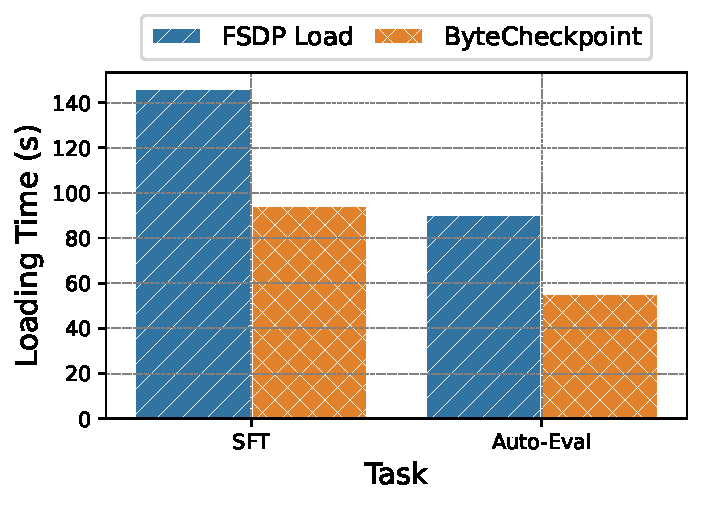
\includegraphics[width=\linewidth]{figures/fsdp_load_resharding.pdf}
%         \caption{DenseGPT 6.7B, FSDP resharding.}
%         \label{fig:fsdp_16_to_8}
%     \end{subfigure}
%     \hfill
%      \begin{subfigure}[b]{0.49\linewidth}
%     \centering
%     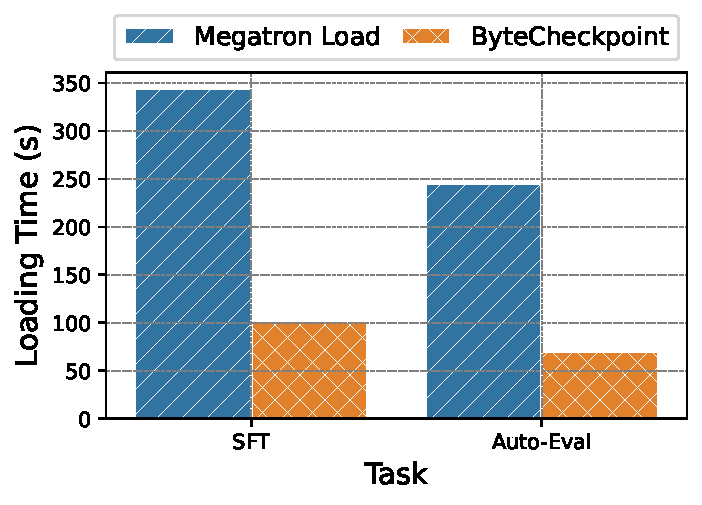
\includegraphics[width=\linewidth]{figures/megatron_load_resharding.pdf}
%     \caption{SparseGPT 28B, Megatron-LM resharding.}
%     \label{fig:fsdp_16_to_24}
%    \end{subfigure}
%     \caption{Resharding efficiency comparison between different methods.}
%      \label{fig:exp_load_compare}
%\end{figure}

%We compare the end-to-end resharding times of different methods on DenseGPT 6.7B and SparseGPT 28B to study %the loading performance of \sys{}.
%As depicted in Fig.~\ref{fig:exp_load_compare}, \sys{} finish checkpoint resharding consistently faster than %baselines.
%Specifically, \sys{} achieves 1.55 $\times$ and 1.62 $\times$ acceleration over FSDP~\cite{fsdp} checkpoint %loading module for SFT and Auto-eval tasks, respectively. 
%These gains are even more pronounced (3.37$\times$ faster on the SFT task and 3.51 $\times$ faster on the %Auto-eval task) when comparing with the loading pipeline of Megatron-LM~\cite{megatron}, which involves the %costly execution of offline resharding scripts.
%Thanks to the zero redundancy loading mechanism, \sys{} can detect unnecessary tensor segments for each %process as well as repeated tensor shards across processes when loading saved checkpoints into new %parallelism configurations.
%It then leverages the partial file reading to avoid redundant segments and overlaps the tensor data reading %with transferring across GPUs, therefore accelerating the whole loading process.

\begin{table}[!t]
\caption{
Saving optimization microbenchmark.
}
\label{tab:save_bench}
\begin{small}
\resizebox{\linewidth}{!}{
\begin{tabular}{c|c|ccc}
    \toprule
    \textbf{Workload} & \textbf{Parallel Config.} & \textbf{Optimization} & \textbf{Saving Time (s)} \\
    \midrule
     \multirow{4}{*}{tGPT 13B } & \multirow{4}{*}{TP=2, DP=8, PP=2} & No Optim. & 50.26\\
     &  & Async. & 34.68 (\textbf{1.45$\times$})\\
     &  & Async. + WB. & 20.28 (\textbf{2.48$\times$})\\
     &  & Async. + WB. + Cache.  & 19.97 (\textbf{2.52$\times$})\\
     \midrule
     \multirow{4}{*}{tGPT 30B } & \multirow{4}{*}{TP=2, DP=8, PP=4} & No Optim. & 46.34\\
     &  & Async. & 25.56 (\textbf{1.81$\times$})\\
     & & Async. + W.B. & 18.83 (\textbf{2.46$\times$})\\
     &  & Async. + W.B. + Cache. & 18.56 (\textbf{2.50$\times$})\\
    \bottomrule
\end{tabular}}
\end{small}
\end{table}

\begin{table}[!t]
\caption{
Loading optimization microbenchmark.
}
\label{tab:load_bench}
\begin{small}
\resizebox{\linewidth}{!}{
\begin{tabular}{c|c|ccc}
    \toprule
    \textbf{Model} & \textbf{Parallel Config.} & \textbf{Optimization} & \textbf{Loading Time (s)} \\
    \midrule
     \multirow{3}{*}{tGPT 13B } & \multirow{3}{*}{TP=2, DP=8, PP=2} & No Optim. & 63.48\\
     &  & Async. & 48.43 (\textbf{1.31$\times$})\\
     &  & Async. + Overlap. & 41.38 (\textbf{1.53$\times$})\\
     \midrule
     \multirow{3}{*}{tGPT 30B } & \multirow{3}{*}{TP=2, DP=8, PP=4} & No Optim. & 77.02\\
     &  & Async. & 74.54 (\textbf{1.03$\times$})\\
     & & Async. + Overlap. & 48.73 (\textbf{1.58$\times$})\\
    \bottomrule
\end{tabular}}
\end{small}
\end{table}

\label{sec:reshard_optim}
\begin{table}[!t]
\caption{
Resharding optimization microbenchmark.
}
\label{tab:reshard_bench}
\begin{small}
\resizebox{\linewidth}{!}{
\begin{tabular}{c|c|ccc}
    \toprule
    \textbf{Model} & \textbf{Parallel Config.} & \textbf{Optimization} & \textbf{Processing Time (s)} \\
    \midrule
     \multirow{2}{*}{tGPT 13B} & \multirow{2}{*}{ZeRO-2 32 GPUs} & All-gather + D2H. & 4.12\\
     & & Decompose. & 0.21 (\textbf{19.80$\times$})\\
     \midrule
     \multirow{2}{*}{tGPT 30B} &  \multirow{2}{*}{ZeRO-2 64 GPUs} & All-gather + D2H. & 5.84\\
     & & Decompose. & 0.19 (\textbf{30.50$\times$})\\
    \bottomrule
\end{tabular}}
\end{small}
\end{table}

\begin{comment}
\begin{table}[!t]
\caption{Resharding configurations.
}
\label{tab:reshard_config}
\resizebox{\linewidth}{!}{
\begin{tabular}{ccccc}
    \toprule
    \textbf{Before} & \textbf{PP} & \textbf{TP}\\
    \midrule
     TP=1, DP=4, PP=4 & TP=1, DP=4, PP=8 & TP=2, DP=4, PP=4 \\
    \bottomrule
\end{tabular}}
\end{table}    
\end{comment}

\begin{comment}
\begin{figure}[!t]
    \centering    
     \begin{subfigure}[b]{\linewidth}
         \centering
         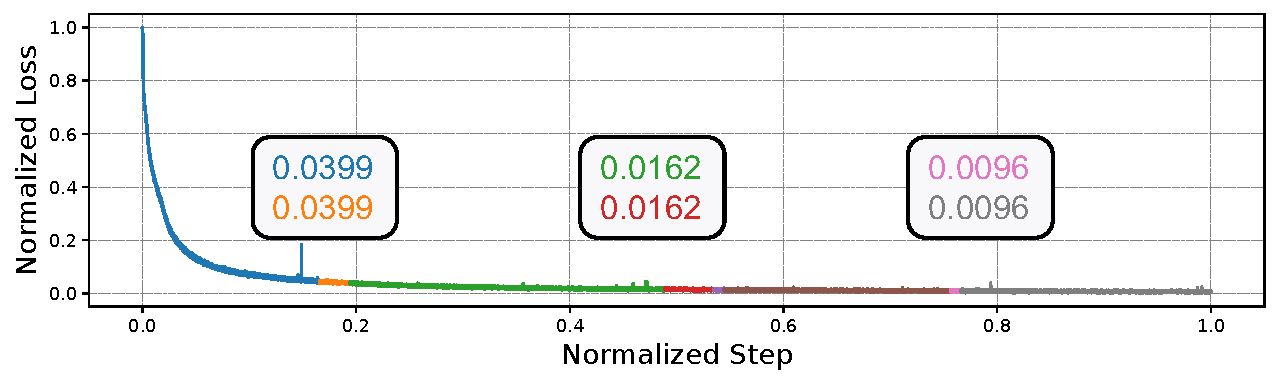
\includegraphics[width=\linewidth]{figures/online_resume_loss.pdf}
         \caption{The normalized loss curve.}
         \label{fig:online_loss}
     \end{subfigure}
     \hfill
      \begin{subfigure}[b]{\linewidth}
     \centering
     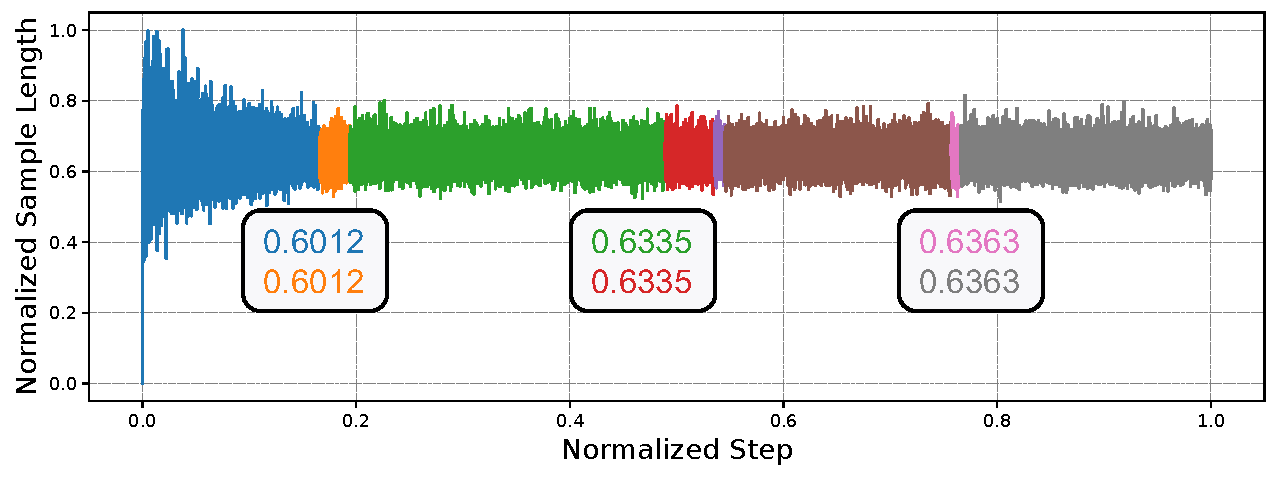
\includegraphics[width=\linewidth]{figures/online_resume_length.pdf}
     \caption{The normalized average sample length.}
     \label{fig:online_len}
    \end{subfigure}
    \caption{
    Training resuming with \sys{} in real production run on 2080 H800 GPUs 
    % \cwu{what type of GPUs?}
    for several days.
    %Different colors 
    Color changes indicate training restarts.
    % \cwu{reduce vertical space taken by the figures}
    }
    \label{fig:exp_online_resume}
\end{figure}    
\end{comment}

\begin{table*}[!t]
\caption{I/O performance of \sys{} in large-scale LFM training.}
\label{tab:io_product}
\begin{small}
\resizebox{\linewidth}{!}{
\begin{tabular}{c|cc|cccc}
    \toprule
    \textbf{Model and Framework} & \textbf{\#GPUs 
    % \cwu{what type of GPUs}
    } & \textbf{Parallelism} & $\mathbf{T_{Block}}$ \textbf{(s)} & $\mathbf{T_{Save}}$ \textbf{(s)} & $\mathbf{T_{Load}}$ \textbf{(s)} \\
    \midrule
     Vision Transformer 7B FSDP & 1488 & ZeRO-2 & 0.34 & 20.13 & 265.73 \\
     Text Transformer 405B Megatron-LM & 8960 & TP=8, DP=70, PP=16 & 0.59 & 51.06 & 129.49 \\
    \bottomrule
\end{tabular}}
\end{small}
\end{table*}

\subsection{Microbenchmarks}
% \yhpeng{Move experiments in Sec.4 to this subsection, TODO: add experiment setup and result description} 
% \zmf{edited at 09/18 15:10 GMT+8}
We conduct several micro-benchmarks (Table~\ref{tab:save_bench}, Table~\ref{tab:load_bench} and Table~\ref{tab:reshard_bench}) to highlight the performance improvements.  To evaluate different model sizes,
We modify the tGPT 70B model to create tGPT 13B and tGPT 30B.
For saving and loading microbenchmarks, we used the Megatron-LM training framework, while for resharding, we employed FSDP.
% The micro-benchmarks tested two workloads, OPT 13B and OPT 30B, with parallel configurations set to TP=2, DP=8, PP=2 and TP=2, DP=8, PP=4, respectively.

In Table~\ref{tab:save_bench}, we compare the end-to-end saving times with and without \sys{} features, as described in Sec.~\ref{sec:io_optimization}.
The results demonstrate that asynchronous saving pipeline achieves significant reduction in saving time compared to the unoptimized settings, yielding speedups of 1.45$\times$ and 1.81$\times$ for tGPT 13B and tGPT 30B, respectively.
The workload balancing mechanism and plan cache of \sys{} can further boost these improvements.
When applying all I/O optimization techniques to both model and optimizer states, the average saving time for these models is reduced from 48.3 seconds to 19.27 seconds.
In Table~\ref{tab:load_bench}, we present the performance gains achieved by the asynchronous loading pipeline and read-communication overlap techniques.
For tGPT 13B and tGPT 30B, the baseline loading times were 1.53$\times$ and 1.58$\times$ longer than those achieved with \sys{}.

% \zmf{edited at 09/18 16:07 GMT+8}
For load-time resharding, we compared the irregular tensor processing time between FSDP and \sys{}'s irregular tensor decomposition strategy. As shown in Table~\ref{tab:reshard_bench}, \sys{} incurs an average blocking time of just 0.20s, which is 25.15$\times$ shorter 
% \cwu{shorter?}
than that of FSDP.
Moreover, our approach consistently achieves microsecond-level blocking times, regardless of the training scale. (see results in Sec.~\ref{sec:exp_main} and Sec.~\ref{sec:exp_product}).
% In stark contrast, the DCP-native approach incurs blocking times of 4.12 seconds (19.80 times longer) and 5.84 seconds (30.50 times longer) for OPT 13B and 30B, respectively.


\subsection{Correctness Verification}
\label{sec:exp_correct}

In Fig.~\ref{fig:reshard_correct}, we depict normalized training loss curves of tGPT 13B before and after resharding with \sys{} in various situations.
%The corresponding parallelism configurations are shown in Table~\ref{tab:reshard_config} \cwu{merge the table information into Fig.~\ref{fig:reshard_correct} to save space}.
For PP and TP resharding, the normalized loss curve after resharding can smoothly match that in the previous phase and continue to display a consistent decline trend.
Unit testing confirms that \sys{} can correctly transform distributed checkpoints across varying parallelism.
% configurations.
% We also give 
Results of DP and hybrid resharding are in Appendix~\ref{sec:exp_full_correct}.

We further verify the bit-wise alignment ability of \sys{} when training resumes without changes in parallelism configurations.
We show the normalized loss curve from real production in Fig.~\ref{fig:online_loss}, where a 175B language foundation model is trained.
% \cwu{what model is trained?}
% Since the RNG state is fixed, correct resumptions should yield the same data sampling trajectory.
% Therefore, we use the normalized data sample length curve (Fig.~\ref{fig:online_len}) to evaluate bit-wise correct resuming of dataloader states.
% \cwu{clarify why data sample length curve can evaluate bit-wise correct resuming of dataloader states}.
As highlighted, the normalized loss before and after resuming are exactly the same.
% Take Fig.~\ref{fig:fsdp_correctness_16_to_8} as an example, specifically, this test comprises two phases: we first apply the ZeRO-2 strategy and train the DenseGPT 6.7B model with 16 GPUs, then save the checkpoints with \sys{}. After that, we resume the training with the ZeRO-3 strategy and reduce the number of GPUs to 8, then load checkpoints from the old configurations.
% Experimental results for the opposite transformation can be found in % Fig.~\ref{fig:fsdp_correctness_16_to_24}.
% Similar findings are observed with the SparseGPT 28B model, which is trained using % Megatron-LM~\cite{megatron}.
% Additionally, we include a scenario without checkpoint resharding % (Figure~\ref{fig:megatron_correctness_no_shard}) to illustrate the broad % applicability of \sys{}. 
% These experimental results confirm the automatic online resharding ability of % \sys{}, which can flexibly accommodate different parallelism configurations and % training frameworks.
\subsection{Checkpointing in Real LFM Production}
\label{sec:exp_product}
We share our experience deploying \sys{} in real-world LFM production environments, highlighting the issues we encountered and resolved.

\noindent \textbf{Scalabilty}.
As shown in Table~\ref{tab:io_product}, \sys{} was used to train two transformer-based LFMs for image and text generation on H800 GPUs, respectively. 
\sys{} consistently maintained average checkpoint stalls under 600ms, even at the largest scale with 8,960 GPUs.
Additionally, end-to-end checkpointings were completed efficiently, typically within a few seconds.
%The online data collected from production environments further underscores the efficiency gains that \sys{} brings to LFM production.

\begin{figure}[!t]
    \centering    
     \begin{subfigure}[b]{0.49\linewidth}
         \centering
         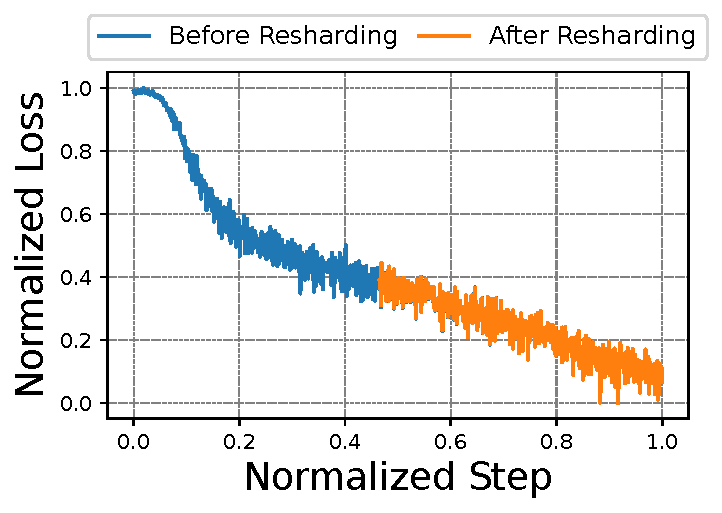
\includegraphics[width=\linewidth]{figures/pp_resharding.pdf}
         \caption{PP resharding from TP=1, DP=4, PP=4 to TP=1, DP=4, PP=8.}
         \label{fig:pp_resharding}
     \end{subfigure}
     \hfill
      \begin{subfigure}[b]{0.49\linewidth}
     \centering
     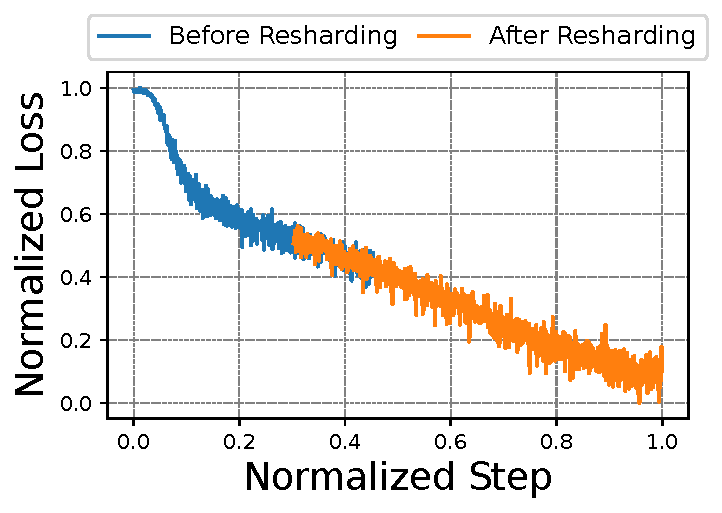
\includegraphics[width=\linewidth]{figures/tp_resharding.pdf}
     \caption{TP resharding from TP=1, DP=4, PP=4 to TP=2, DP=4, PP=4.}
     \label{fig:tp_resharding}
    \end{subfigure}
     \caption{Resharding correctness verification. 
     % \cwu{increase font size along x, y axes and legends in the figures}
     }
      \label{fig:reshard_correct}
\end{figure}

\begin{figure}[!t]
  \centering
  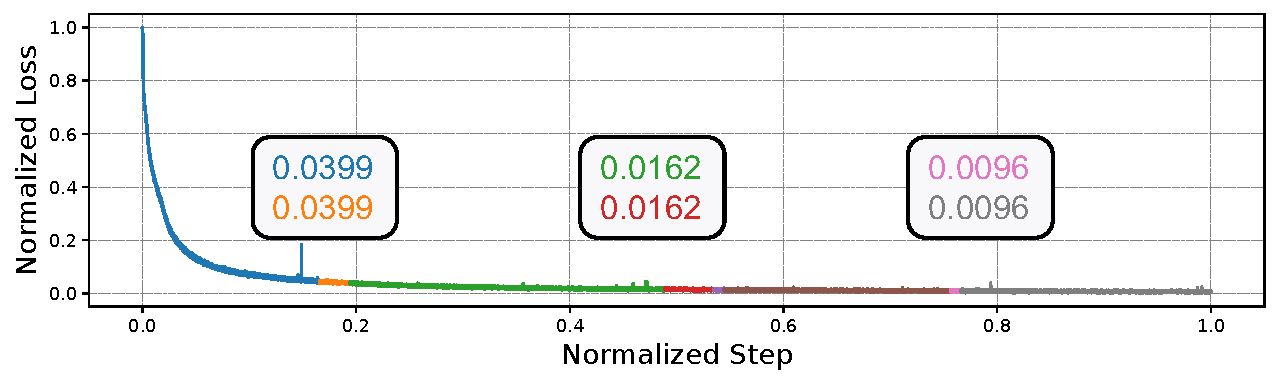
\includegraphics[width=\linewidth]{figures/online_resume_loss.pdf}
  \caption{
    Training resuming with \sys{} in real production run on 2080 H800 GPUs 
    % \cwu{what type of GPUs?}
    for several days.
    %Different colors 
    Color changes indicate training resuming.
    % \cwu{reduce vertical space taken by the figures}
  }
  \vspace{-5mm}
  \label{fig:online_loss}
\end{figure}

\noindent \textbf{Dataloader stragglers}. 
% \yhpeng{@mofan visualization helps us detect some stragglers caused by dataloaders. and how we optimize dataloader ckpts.}
% \zmf{edited at 9/17 19:56 GMT+8, @yiyao and @borui to refine and condense this section}
By analyzing the performance visualization results from our monitoring tools (Sec.~\ref{sec:visualization}),
% we identify that the uploading of dataloader checkpoint files imposes significant overhead on a few ranks, leading to a pronounced long-tail latency issue. 
we identified prolonged uploading time for dataloader checkpoint files.
% Specifically, in large-scale pre-training tasks using Megatron-LM, only % those GPU ranks where both the tensor parallel and pipeline parallel rank indices are 0 are responsible for saving dataloader checkpoints. This subset represents only a small fraction of the total GPU ranks. 
% Unlike model or optimizer checkpoints, which balances across all GPU ranks by \sys{}, dataloader checkpoints involve a larger per-rank volume, potentially reaching the GB level. 
To support dataloader state resharding, \sys{} divides the states of a dataloader into multiple parts (e.g., 6 parts for the tGPT experiments in Sec.~\ref{sec:exp_main}) and stores them as individual files.
These files can be independently loaded during resharding.
However, uploading these small files sequentially leads to low bandwidth utilization, causing performance degradation. %leading to 
% \cwu{clarify what is long-tailed - the distribution of uploading time? if there is no distribution involved, call it prolonged uploading time instead}.
In cases like the 7B vision transformer, uploading time of dataloader states can account for 73.16\% of total saving time.
% \cwu{tell what the scenarios are in the production experiments},
To fix this issue, we implemented a process pool for concurrent uploads, significantly reducing saving time.
% rather than following the sequential pipeline approach.
% Moreover, since the dataloader checkpoint files are already partitioned, we distribute the saving and uploading workloads across ranks within the same DP group.

\noindent \textbf{HDFS metadata bottleneck}. %\yhpeng{Add problems discovered and fixed in production.} \zmf{edited at 9/17 20:59 GMT+8}
Through monitoring, we identified several bottlenecks related to HDFS. Despite applying the parallel optimization techniques for single-file uploads described in Sec.~\ref{sec:io_parallel}, the actual HDFS upload performance fell short of our expectations.
A detailed profiling revealed that the metadata concatenation operation in the HDFS NameNode was performed serially, making it a significant performance bottleneck when large volumes of checkpoint files were generated. We mitigated this issue by enabling parallel execution of the concatenation operation.
Another issue that emerged was related to our initial use of the HDFS SDK.
For the convenience of the users, the SDK encapsulates a lot of safeguard logic, leading to unnecessary overheads introduced by checking, creating parent directories, and verifying target files.
To address this, we optimized \sys{} by ensuring directory existence and file uniqueness prior to invoking HDFS APIs, reducing redundant metadata operations and improving performance significantly.
By addressing these issues, we reduced the maximum metadata overhead of HDFS write operations for a single checkpoint file from 3s to  150ms.
